\chapter{Foundations}
This chapter illustrates the basic principles of \nameref{sec:cloud-computing}, \nameref{sec:tex} and \nameref{sec:collaborative-software}. Additionally, it focusses on the specialities of \nameref{subsec:collaborative-editing-foundations}, the as well as the \nameref{subsubsec:operational-transform} algorithm in theory, practice and the necessary knowledge for the implementation of undo and redo with it.

\section{Cloud Computing}
\label{sec:cloud-computing}

An overview over the theoretical foundations, underlying principles and technologies of Cloud Computing will be given in this chapter. It starts with a brief introduction to the characteristics and is then looking at the different deployment and service models of Cloud Computing, \nameref{subsubsec:iaas}, \nameref{subsubsec:paas} and \nameref{subsubsec:saas}. 

Regarding these service models, the infrastructure of the Institute of Telematics' private cloud will be briefly outlined afterwards, before ending the chapter with basic foundations of collaborative software and the specifics of collaborative editing, including standard algorithms.

\subsection{History}
\label{subsec:cloud-history}
The history of Cloud Computing is inseparably connected to the one of large-scale computing in computer science and can be viewed as a wavelike expansion over time. It started with rapid initial growth, then went into decline and is now surging to new heights.

\begin{figure}[h!]
	\centering
		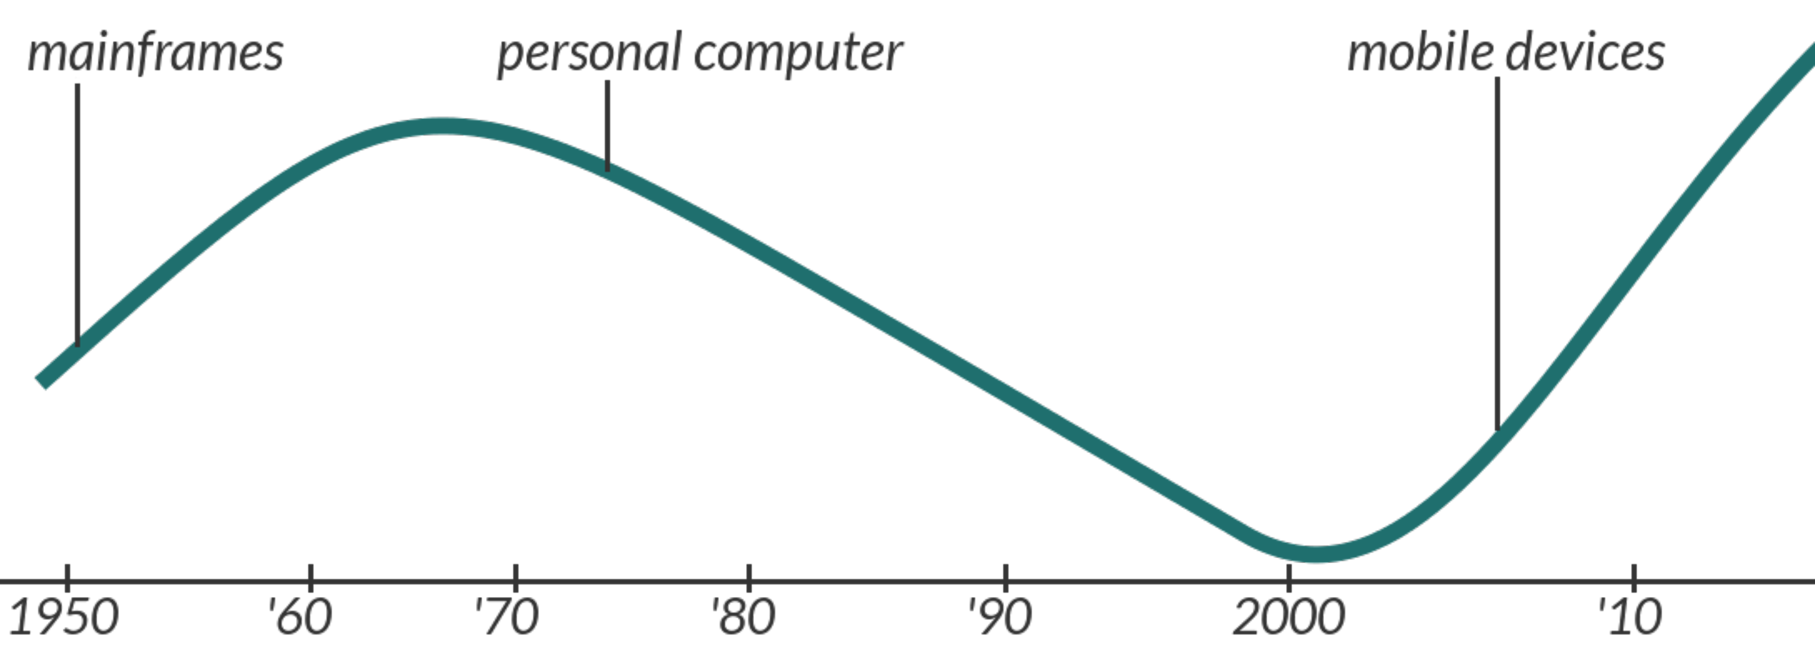
\includegraphics[width=0.8\textwidth]{images/computing_expansion.pdf}
	\caption{History and prevalence of large-scale computing over the decades}
\end{figure}

In the early days of computing, the 1950s and 1960s, large-scale mainframe computers where used in public constitutions such as universities, military research facilities and business companies around the globe, commanding them on terminals. In that period, they reached their all-time peak for the time being and in the following decades, the success of the personal computer led to their steady decline and the belief, that the future of computerisation is personalised. This is turning out to be very true. 

The roaring growth of the Internet and its ubiquitous use on mobile devices gave large-scale computing a comeback, with data centers nowadays representing the backbone of major Internet companies and enabling recent technological approaches like Big Data or Cloud Computing.

In the foreseeable future, this development is even going to speed up as more and more people are connected to the Internet and previously local applications for the computer are now being provided as services and shifted into the cloud, for instance Photoshop, which is now available only via the Adobe Creative Cloud \cite{website:adobe-shift-cloud} \cite{website:adobe-photoshop-cc}. But the pioneers of Cloud Computing where other companies.

The rise of Cloud Computing can be seen as an aftermath of the New Economy. After its demise, companies had to reinvent themselves to survive the struggle for customers and draw several lessons from it \cite{bitkom2012soacloud}:

\begin{itemize}
	\itemsep2mm
	\item{Competition is universally in the Internet and each competitor is always just a single click away. Customers are product- and not vendor-loyal, always on the look for the most innovative, easy to use and especially cheap provider. Such with comfortable, attractive and intuitive user interfaces have a competitive advantage.}
	\item{Customers are very sensible to fluctuations in the quality of service. Amazon had to learn that a 1/10 of a second slower response time can already lead to a decrease in revenue by 1\%, while Google noticed the same for search requests, with a 20\% drop if response times slowed down by 0.5 seconds.}
	\item{If a product will find a ready market, demand exceeds supply rapidly and only massive-parallel IT infrastructures have the potential to scale accordingly on short notice. Software must developed agile and interchangeability of a component-based software architektur is a must, making permanent innovation possible.}
\end{itemize}

Google and Amazon where the first companies to react to these new challenges, both in their own way.

After the end of the boom, companies had difficulties to acquire money for their growing businesses, as angel investors were cautious and venture capital has become scarce. Google adapted to it by using only hardware from low-budget computers, interconnecting them to a heterogenous, massive, parallel computing archictecture, promising endless extensibility. 

\pagebreak

Using this type of infrastucture resulted in several non-trivial problems, as parallel architectures can merely scale if software components share nothing, and Google solved them by software \cite{lee2011sharednothing}. For this, a particular database \name{Google Big Table} was developed as well as fault-tolerant software, leading to the invention of the established \name{MapReduce} algorithm \cite{dean2004mapreduce}. 

This infrastucture emerged to be extremely cost-efficient and was copied by various other companies, nowadays being the blueprint of massive-parallel architectures and Cloud Computing.

Contrary to Google, Amazon was part of the Internet boom and invested enormously into its infrastructure during that time, building up huge, unused capacities. To make use of its bloated infrastructure, Amazon decided to rent it out to other companies. This move, initially being born out of pure economical necessity, made Amazon the first real service provider, awarding itself with a lucrative revenue stream besides its main business. But unknowingly, it also laid the second cornerstone for Cloud Computing. 

In the wake of early success, Amazon constantly evolved the new business model and formed an independent branch with cloud services, now known as \name{Amazon Web Services} (\abk{AWS}{Amazon Web Services}), which today significantly contributes to the company's operating income.

The aforementioned developments, made by both companies independently of each another, transformed the IT landscape permanently as others learned how to use Google's and Amazon's game changing ideas for their purposes which led to the creation of the Cloud Computing industry.  

At that time, the term Cloud Computing was also coined. It derives from the common practice to model the Internet as a cloud-shaped drawing in network diagrams \cite{hausman2013cloud}.

\subsection{Standards and Characteristics}
\label{subsec:cloud-standards}
While Cloud Computing is ubiquitously used nowadays and considered an industry standard, no distinct and universal definition emerged over the years. However, the United States National Institute of Standards and Technology (\abk{NIST}{National Institute of Standards and Technology}) published a definition in 2011 that is widely regarded as most important publication on this topic and effectively considered as reference standardisation \cite{mell2011nist}. 

Following the publication of the definition, the NIST layed out a road map for the creation of an official standard, which was published in July 2013 in its most recent version and contains contributions from members of the NIST themselves as well as other universities and several industry partners such as Oracle or Microsoft \cite{sokol2013nist}. Furthermore, a conceptual reference architecture was published in 2011, which defines not only roles, technological and architectonic aspects, but also quality and orchestration of services. 

\begin{figure}[H]
	\centering
		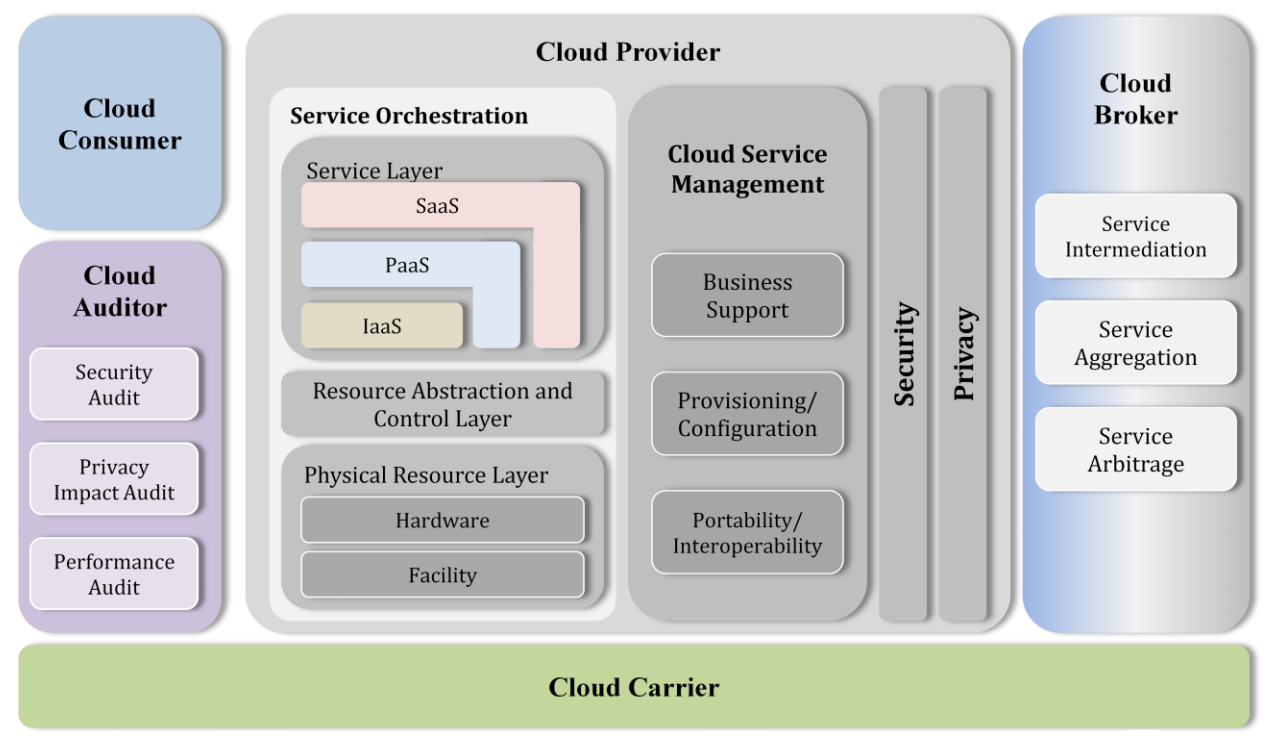
\includegraphics[width=0.85\textwidth]{images/cc_conceptual_reference_model.png}
	\caption{The conceptual reference model of the NIST \cite{liu2012reference}}
\end{figure}

As this broad approach aims to cover for all possible platforms and conceivable uses, there will only be a brief explanation of the most important parts of the reference architecture for this work, which essentially condenses to \name{Services Orchestration}. That term refers to the coordination and management of software and hardware resources for the provisioning of holistic cloud services to consumers.

\begin{figure}[H] % \todo{vor Druck ändern -> h!}
	\centering
		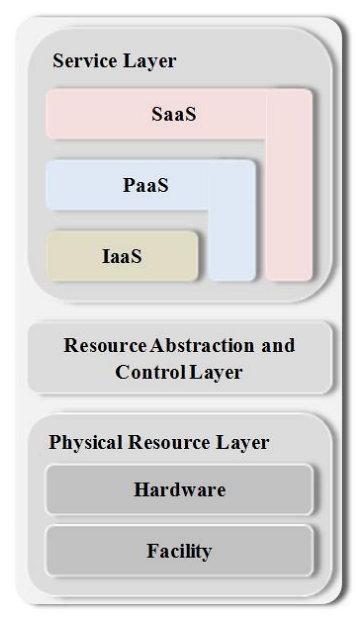
\includegraphics[width=0.275\textwidth]{images/cc_reference_part.png}
	\caption{For this work relevant part of the conceptual reference model of the NIST \cite{liu2012reference}}
\end{figure}

The \name{Services Orchestration} model consists of three different layers, the \textit{service layer}, the \textit{resource abstraction and control layer} and \textit{physical resource layer}, expressing the dependency and abstraction between these. From top layer to bottom layer, each component bases on the one from the contiguous lower layer, while the one's from the lower layers cannot directly access the one's above them.

Representing the top of the model, the \textit{service layer} is defining the interfaces that cloud consumers interact with when they are using cloud services. The single layers are explained profoundly in chapter \ref{subsec:cloud-service-models} in the section \nameref{subsec:cloud-service-models}. Regarding this model however, it is necessary to know that it is possible but not required that the layers are built on top of one another, therefore these are shown as components stacking on each other while being seperate layers. That way, a \nameref{subsubsec:saas} can either be built on top of a \nameref{subsubsec:paas} or hosted on a self-provisioned infrastructure.

The middle layer, \textit{resource abstraction and control layer}, contains system components that providers use to let others access the underlying physical resources. It ties together the various resources and their software abstractions and serves as middleware. The additional \textit{control} aspect refers to access control, monitoring and usage supervision.

The \textit{physical resource layer} includes generally all hardware related infrastructure and resources but exceeds the simple provisioning of CPUs, memory and data store by far. It also involves all physical elements such as power, cooling, maintenance and other aspects.

Given this model and it's layers, only the first can be considered really relevant for this work, as the final application will be a \nameref{subsubsec:saas}, relying on other technologies and middlewares, such as OpenStack, managing the physical resource layer. Although the other layers are used as well, they are much less of a concern, only abstracting resources for the top layer on the sake of easier utilisation.

As previously stated, a definition of Cloud Computing was published by the NIST in 2011 and it also stated five main characteristics, namely \textit{on-demand self-service}, \textit{broad network access}, \textit{resource pooling}, \textit{rapid elasticity} and \textit{measured service} \cite{mell2011nist}. \\
While these characteristics are universally applicable, their composition is rather theoretical and there are some aspects missing. For this reason, they are complemented and extended in the following. This is also showing that Cloud Computing shares most characteristics with distributed systems, but has some unique qualities that distinguishes it from other approaches and underlines its superiority towards them.

\begin{description}
	\itemsep2mm
	\item[Agility] \hfill \\
		The flexible provisioning of any resources needed by the customer, offering web interfaces to dynamically self-manage the utilisation of provided services.
	\item[Device Independence] \hfill \\
		Customers must be able to access cloud services with any device, be it laptop, tablet or mobile phone.
\pagebreak
	\item[Application Programming Interface (\abk{API}{Application Programming Interface})] \hfill \\
		Accessibility has not only to be provided for developers but computers as well by creating machine-readable interfaces. Such an API will typically be implemented using Representational State Transfer (\abk{REST}{Representational State Transfer}).
	\item[Costs] \label{item:costs} \hfill \\
		Costs are one of \textit{the} benefits of Cloud Computing and the major sales argument for providers. Previously, an organisation or business had to maintain its own complete IT infrastructure, which was then in fact mostly unused as the available capacity also reflected necessary reserves to meet peaks in demand. Moreover, such an infrastructure meant having dead capital that could not be spent elsewhere. With Cloud Computing, this money is freed-up for businesses, being able to use it on other spendings while having only to pay for the actual use of IT infrastructure and/or services.
	\item[Geographical Diversification] \hfill \\
		Major service providers operate data centers on different locations, often spread over the whole world and all continents. When provisioning their services, the nearest to the customer located site will be chosen to handle all requests, accounting for minimal response times and higher quality of service.
	\item[Virtualisation] \hfill \\
		Targeting to utilise hardware in the most optimal way, it allows infrastructure such as servers and storage to be shared. Virtual machines are abstracting the hardware layer, allowing software to be executed on any host without restraints. This is done by emulating the underlying hardware resources purely in software. That way any guest can be used on any host, running virtual machines with Linux on Windows hosts or the other way around. This is essentially when migrating applications in the form of virtual machines between servers, which is a must for scalability and load balancing.
	\item[Multitenancy] \hfill \\
		Multitenancy is the actual effect of virtualisation, as it means sharing resources and costs amongst multiple service customers. It reflects the centralisation and better average utilization of infrastructure, as explained earlier in Costs.
	\item[Reliability] \hfill \\
		Realiability is not only meant in such a way that provided services are reachable 24 hours a day, seven days a week, but that they also come with absolute fault tolerancy, guaranteeing a 100 per cent uptime for business continuity.
	\item[Elasticity] \hfill \\
		As it is closely related to scalability, it defines the degree to which a system can adapt to changing loads and peaks, dynamically provisioning resources when needed and deallocating them when not. This intelligent load balacing differentiates it from the term scalability, which describes only the scaling itself but not automation of doing so.
	\item[Monitoring] \hfill \\
		Performance, use of services and system errors are monitored. The first one is done for customers to see their systems performance but also for the provider to optimise its systems effencience as well as finding possible faults like memory leaks. The second is used to bill the services and the last to react to failures.
	\item[Security] \hfill \\
		Non-disclosure of a customers data is imperative, as well as guaranteeing their integrity and protection against data loss. These concerns are even more urgent in a multi-tenant environment, as it exists in Cloud Computing. At the same time several Cloud Computing characteristics, e.g. distribution, add to complexity and increase the difficulties of securing these systems.
	\item[Maintenance] \hfill \\
		Maintenance is a cross-cutting concern to assure several, previously mentioned characteristics of Cloud Computing like security, performance and reliability. This can only be achieved when hardware replacements or software updates are completely transparent to the customers.
\end{description}

\subsection{Deployment Models}
\label{subsec:cloud-deployment-models}
When speaking of clouds, publicly available services of large Internet companies come to mind, but it is not imperative for clouds to be public. They can also be private, even so partially, which then makes a hybrid model, as can be seen in the following descriptions.

\begin{description}
	%\addcontentsline{toc}{subsubsection}{Public Clouds}
	\item[Public Clouds] \hfill \\
		Available to the general public, they are owned and provisioned by businesses or organisations, sharing their resources over the Internet, involving web applications and often third-party tools. When billing them, it will be on a per-use basis.
	%\addcontentsline{toc}{subsubsection}{Private Clouds}
	\item[Private Clouds] \hfill \\
		Contrary to the above, a private cloud exists only within the enterprises' or organisation's boundaries, being shielded from the Internet by internal firewall. As most benefits and characteristics of public cloud are shared, this self-management is the major distinction between them.
	%\addcontentsline{toc}{subsubsection}{Hybrid Clouds}
	\item[Hybrid Clouds] \hfill \\
		The combination of public and private clouds, dividing responsibilities between the company or organisation and service provider, is called hybrid. It can be composed of two or more clouds that are their own entities but bound together. Hybrid clouds are often used to ensure privacy, integrity and safety of data by storing them in-house, while relying on public cloud providers for less critical data and services.
\end{description}

\subsection{Service Models}
\label{subsec:cloud-service-models}
With the continuing development and growing maturity of Cloud Computing, lines between the different service models are beginning to fade more and more. Nowadays there is an approach to provide Everything as a Service (\abk{XaaS}{Everything as a Service}), but when looking at Cloud Computing as a stack, there are three different service models that have evolved over the time, depicted by the following graphic. For the sake of completeness and better understanding, clients have been added to it as well.

\begin{figure}[H] % \todo{vor Druck ändern -> h!}
	\centering
		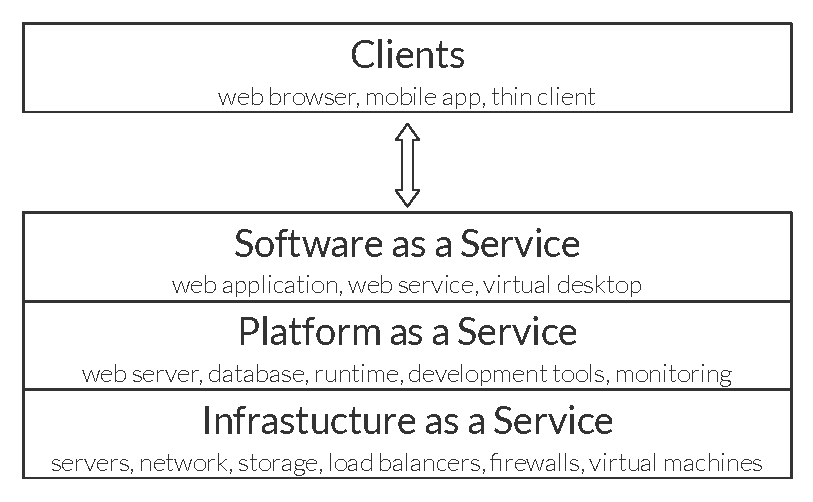
\includegraphics[width=0.66\textwidth]{images/cc_service_models.pdf}
	\caption{The three service models of Cloud Computing}
\end{figure}

While each service model can be used independently and does not require to utilise the underlying model to tender its services, providers often rely on them for reasons of simplification and cost effectiveness. Therefore making it an actual stack, when other as-a-Service's are used.

\subsubsection{Infrastructure as a Service}
\label{subsubsec:iaas}
Being the most low-level of the three service layers, Infrastructure as a Service (\abk{IaaS}{Infrastructure as a Service}) is the cornerstone of Cloud Computing architecture and provides for all hardware needs. It typically includes the provisioning of servers, storage, firewalls, load balancing, interior and exterior network connectivity \cite{mcgrath2012understanding}. In addition to it, all dependent services like monitoring, security, maintenance, but also intangible assets as knowledge and personnel will be taken care of by providers, leaving the service consumer with very few residual tasks on his own.

Major providers also possess geographically diversified services, meaning that a host serving a request will be dynamically chosen in the nearest data center to the service consumer.

\pagebreak

Regarding the technology, Infrastructure as a Service involves not only physical computers but even more so virtual machines, allowing multiple guest systems to share a host and dynamically allocating ressources when needed, therefore reducing costs. The costs are based on the actual resource allocation and consumption, typically ranging from a couple of cents to several dollars per hour \cite{website:aws-ec2-pricing}.

A detailed consideration of underlying technologies can not accomplished this work. Therefore related topics like virtualisation, hypervision, compute instance, resource pooling and so forth will not be addressed further, as the reader is assumed to research these on his own.

\subsubsection{Platform as a Service}
\label{subsubsec:paas}
Providers of Platform as a Service (\abk{PaaS}{Platform as a Service}) offer, as they name states, a platform for others to use. This is more abstract to define than the other service models, but essentially this amounts to the task of provisioning everything it takes to run a specific programming language or technology stack \cite{mcgrath2012understanding}. Typically this includes web server, database, runtime environment, development tools, monitoring. 

This may seem trivial at first. For developing Java applications, for instance, not much more than the \name{Java Development Kit} (\abk{JDK}{Java Development Kit}) including the \name{Java Virtual Machine} (\abk{JVM}{Java Virtual Machine}) and an application server like \name{Tomcat} or \name{Glassfish} is needed, but there are several tasks as dependency management, configuration, maintenance and monitoring to it. It will need to run on an operating system, which will most likely be virtualised as well, relying on the aforementioned \nameref{subsubsec:iaas} or hosted by the provider himself. The complexity of all these challenges are encapsulated by the PaaS provider, being responsible for the immaculate service availability.

Having virtualisation serving as a model where several images can share a host, PaaS providers nowadays do the same within these virtual machines and allocate several applications from different customers, creating a more economic multi-tenant infrastucture.

Platform as a Service also relies heavily on using and serving web solutions, where it can play out it's strengths. \abk{HTTP}{Hypertext Transport Protocol} requests are short-living processes and can be distributed evenly to exisiting servers where they will be processed and then replied to. This is lesser the case for longer running, more resources-demanding jobs, making it not as reasonable to let them run on PaaS environments.

\subsubsection{Software as a Service}
\label{subsubsec:saas}
Software as a Service (\abk{SaaS}{Software as a Service}) is the form of Cloud Computing most commonly known in the general public. Any person being on the Internet will likely have seen it, as all major internet companies provide hosted software for on-demand use. 

\pagebreak

It is typically in the form of an web application, but may also be a web service, a virtual desktop and so on, meaning it is accessed by web browser or thin client. Therefore SaaS can be used from anywhere, anytime, as the only requirement is a working Internet connection.

Using hosted software has multiple advantages. First off, there is no need for customers to install software if they want to use it, it is readily available in the cloud. The same applies for updates, as the service provider always maintains the most recent version of his product. So there is no need for maintenance or support on the customers side, both will be done by the provider. When hiring new staff, the organisation or business will simply need to acquire new licenses, in contrast to the accustomed model where IT has to set up a new employee's computer with all the necessary software and settings \cite{hausman2013cloud}.

This results in total scalability of the applications and the rather sophisticated work behind it is transparent to the customer. When scaling applications, backstage processes first involve cloning and reallocation of virtual machines, then load balancers distribute the tasks to them. Multi-tenancy - as already briefly described in \nameref{subsubsec:iaas} - is broadly used for it as well.

\section{Collaborative Software}
\label{sec:collaborative-software}
Software is described as collaborative if it was designed with the intention to let people work together and achieve common goals, which is sometimes also referred to as Groupware \cite{johnson1990rhythms}. It was defined by Ellis, Gibbs and Rein in 1991 as:

\begin{quote}
	computer-based systems that support groups of people engaged in a common task (or goal) and that provide an interface to a shared environment \cite{ellis1991groupware}
\end{quote}

Its origins can be traced back to the early 1960s when it was envisioned by human-computer interaction and Internet pioneer Douglas Engelbart, who presented it then on the Fall Joint Computer Conference 1968 \cite{engelbart1962conceptual} \cite{engelbart1968human}. This presentation was retrospectively called the \name{Mother of All Demos} as it showcased myriads of inventions that found their way into modern computing. It featured the first computer mouse, a network computer system with real-time text editing and hyperlinks, document version control, a graphical user interface with multiple windows, a predecessor of video conference called teleconference and some more \cite{website:engelbart-1968demo}. When it was connected to the Advanced Research Projects Agency Network (\abk{ARPANET}{Advanced Research Projects Agency Network}) the following year, the first precursor of modern collaborative systems gained an even larger user basis.

Since computer's hardware and connectivity was not ready yet to introduce these developments for personal use and to the general public, more research was conducted, in academia as well as in free enterprise and applications as online chat, video sharing and more were developed further over the next decades.

\pagebreak

With improved technical developments and enhanced maturity of these applications, collaborative software was started to be taken seriously in the beginning 1990s and introduced by the United States government, mainly for military usage. It was also around that time when \name{Lotus Notes} became the first major enterprise application to feature group collaboration and was introduced by several big companies, for instance Pricewater House \cite{website:notes-history}.

As collaborative software was continuously evolving, its next logical step was the migration to the Internet, actively playing a part in the creation and development of what is now known as \name{Web 2.0}, which featured sharing and collaboration as its central resources. That way document sharing, group calendars, instant messaging and video conferencing, amongst other things, were incorporated into applications and websites for the first time and became available to the common user.

\subsection{Collaborative Editing}
\label{subsec:collaborative-editing-foundations}
Collaborative editing is an area of collaborative software where people work together on a problem by making individual contributions. It is divided into several sub-tasks and those are then assigned to either a single person or multiple persons who will work together on one or more tasks.

Such projects are typically more complex in their volume and extent, as is the process of its creation, because collaboration requires coordination between all involved individuals. Besides the actual writing, its structure and the work flow amongst individuals must be also planned and revised and is generally discussed by the whole group.

Collaborative editing is mostly applied for textual documents or source code, asynchronously or in real-time. Such examples for asynchronous collaboration are Wikipedia or version control systems, while Google Docs for instance facilitates real-time collaboration on textual documents. Access management and authentification is essential in both cases but the latter requires even more sophisticated software assistance. 

This software can be a traditional desktop applications, like version control systems, but nowadays more and more applications were migrated to the Internet and are now provided as web applications, like Google Docs. The major technique behind the support for collaborative real-time editing is Operational Transform, which will be explained in the next section.

\subsubsection{Operational Transform}
\label{subsubsec:operational-transform}

Operational Transform (\abk{OT}{Operational Transform}) is the technology for the support of collaborative functions in software systems. It was invented more than two decades ago by Gibbs and Ellis for their GROVE (GRoup Outline Viewing Edit) system and originally designated for the concurrency and consistency control of collaborative editing of text-based documents \cite{ellis1989ccigs}. \\ Nowadays, its collaborative aspect is not limited anymore to the editing of text. As the technology evolved, so did its applications. 

By now it is used for various other tasks as drawing or solving a Rubik's Cube in real-time \cite{website:io2013-drive-api-video}. But capabilities for text-based operations also increased dramatically. Now there is undo, locking, conflict resolution, notifications, sharing and more. It is the core technique behind collaboration features of several major products like Apache Wave or Google Docs.

First, Operational Transform is explained in theory, then an example from real life given and walked through. At last, the specifics of undo and redo operations with Operational Transform are reviewed.

\headline{Theory}
\label{subsubsec:ot-theory}

The foundation of Operational Transform are operations: An action which is to be performed on a data structure - although here it will be focussed on documents. Performed operations on documents are called mutations. The fundamental operations are \method{insert}, \method{delete}, \method{retain} and are more or less self-explanatory. They are used to insert characters, delete characters and move the index by so and so many positions ahead before applying the next mutation.

To handle the concurrent execution of these operations, there is something called \name{transform}, a function that takes two operations, that have been applied on the same document but in different states, from two clients. It re-computes the second operation so that the intended changes of the first operation are preserved and incorporated into the second operation, which can then be applied correctly after taking the first operation into account.

To make this more comprehensible, an extensive example shows the concurrency problems that can appear and the application of Operational Transform to solve them.

\headline{Practice}
\label{subsubsec:ot-practice}

When inserting and deleting locally, it poses no problem to execute these operations as there are no dependent and concurrent operations from other clients that need to be applied.

\begin{figure}[H] % \todo{vor Druck ändern -> h!}
	\centering
		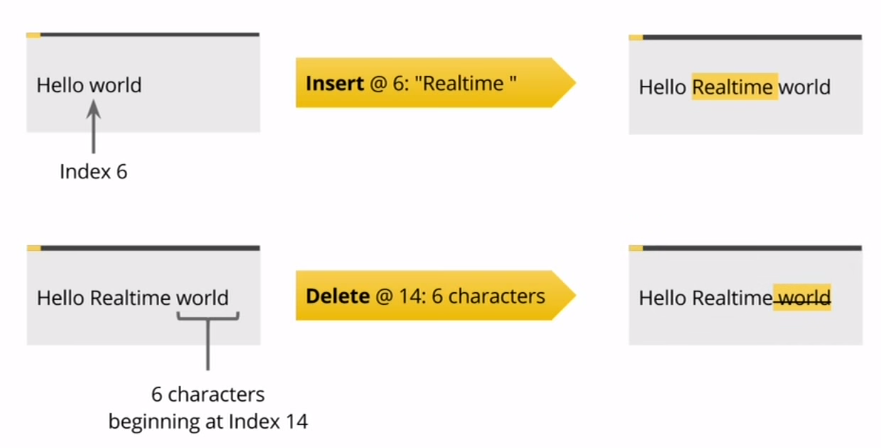
\includegraphics[width=0.75\textwidth]{images/ot_local_insert.png}
	\caption{Local insert and delete of characters \cite{website:io2013-drive-api-video}}
\end{figure}

Synchronising these single local changes between multiple clients is however where problems arise. While editing the same document concurrently, they cannot be simply applied in the order how they would have been locally. This can be seen on the left side of the graphic below. As the second operation is inserted with the local index of the other client, the mutation messes up the document and leaves it in an incorrect state.

The index of the second operation needs first to take the initial operation into account, offsetting its index by the length of the first insert. The re-computed second operation with the altered index position can then be applied correctly, as seen on the right hand side of the graphic below.

\begin{figure}[H] % \todo{vor Druck ändern -> h!}
	\centering
		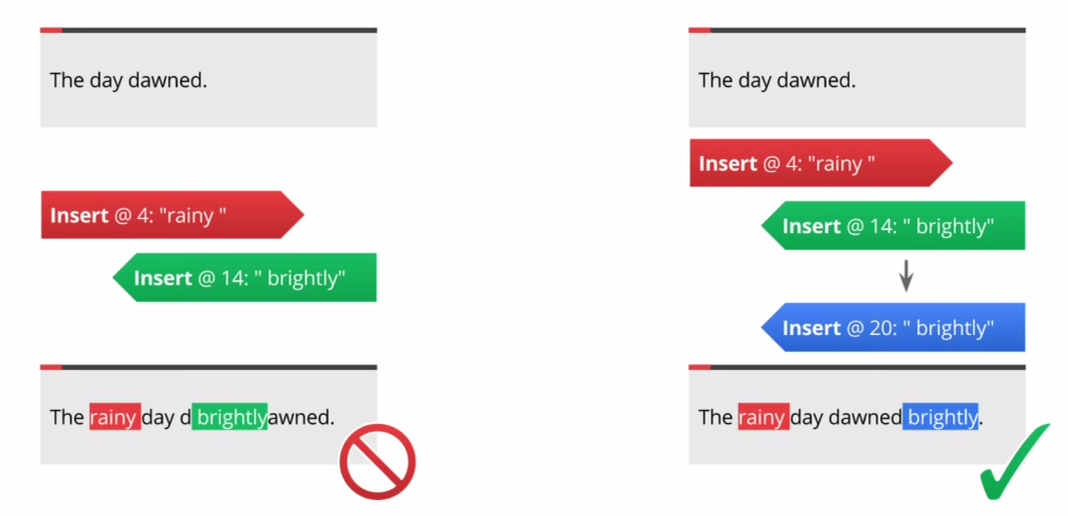
\includegraphics[width=0.85\textwidth]{images/ot_transform_insert.png}
	\caption{Local changes get out of date when other user's changes are incorporated \cite{website:io2013-drive-api-video}}
\end{figure}

What adds to complexity is the transit time of messages. It can lead to further problems when the server, ensuring the transform of operations, is receiving the operations of one client after the ones of another. While all operations can be correctly applied on the client that was sending its operations first, they cannot be on the client whose message reached the server later. Consistency is not achieved in this case.

The problem lies in the processing and transform of operations by the server only. To reflect varying message transit times and being able to handle any incoming operations correctly, regardless of their order and delay, the \name{transform} algorithm also needs to be applied locally. The client must therefore implement the algorithm as well.

\begin{figure}[H] % \todo{vor Druck ändern -> h!}
	\centering
		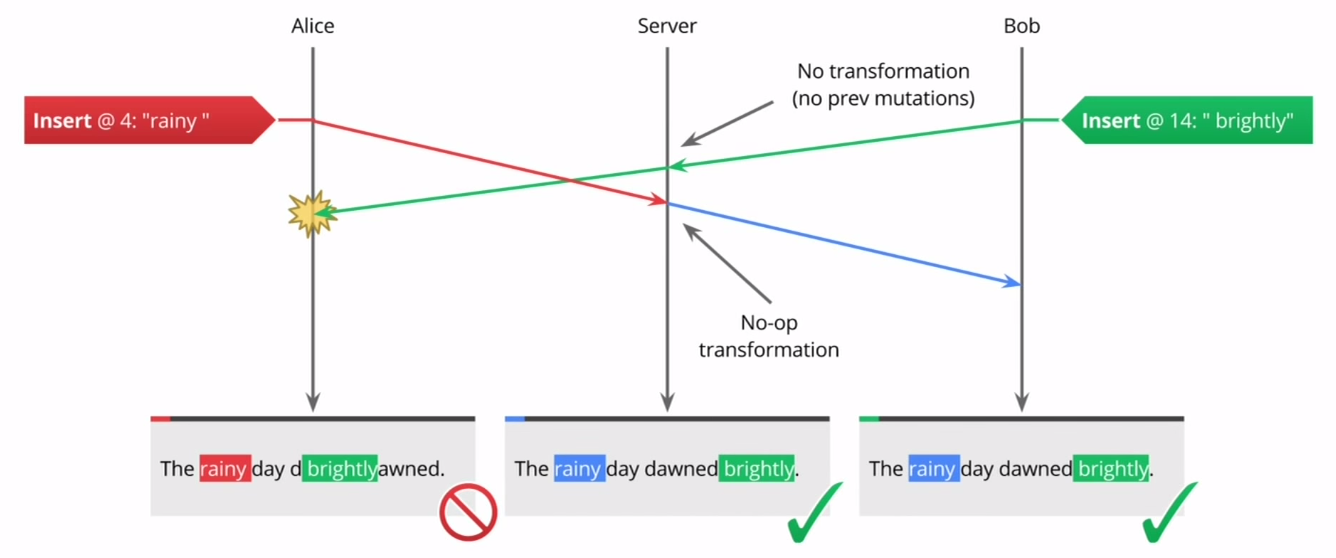
\includegraphics[width=\textwidth]{images/ot_message_transit.png}
	\caption{Conflicts arise when different user operations are performed one after another and their position marks are out-dated \cite{website:io2013-drive-api-video}}
\end{figure}

\headline{Undo and Redo}
\label{subsubsec:ot-undo-and-redo}

For the support of undo and redo of changes made to the document, all operations are pushed to a stack. This holds true for the ones made by the local client as well as those from other collaborators, tracking local and remote changes. The difference however is, that while collaborators' changes are stored unaltered, local changes must be stored with their inverse. For instance, the inverse of an \method{insert} is a \method{delete} and vice versa the inverse of a \method{delete} is an \method{insert}.

\begin{figure}[H] % \todo{vor Druck ändern -> h!}
	\centering
		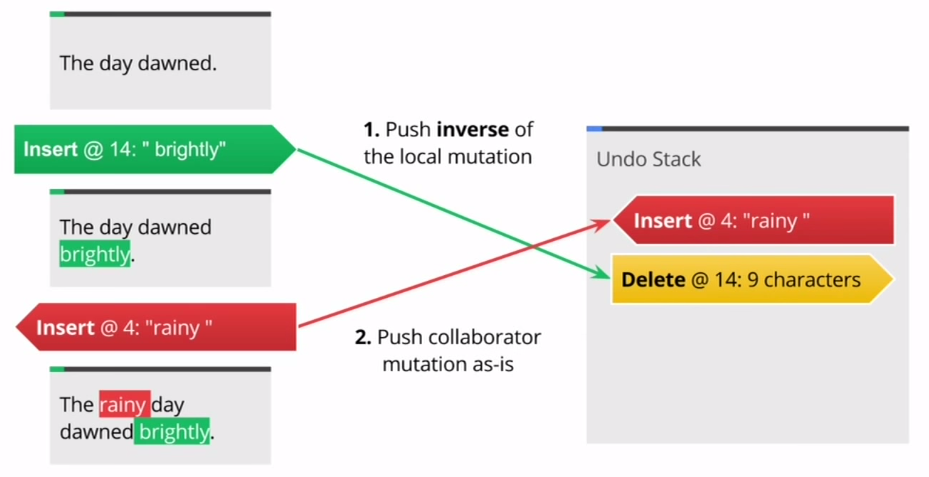
\includegraphics[width=0.75\textwidth]{images/ot_redo_stack.png}
	\caption{All changes are stored on a stack to undo operations in correct order \cite{website:io2013-drive-api-video}}
\end{figure}

\pagebreak

The actual operations and their order on the stack are reasoned by the following: To realise the undo operation, first all collaborator operations are popped from the stack until a local operation is found. The local operation (which is again, the stored inverse of the original operation) must then be transformed against the collaborator's operation to update its index, here shifting it by six positions.

\begin{figure}[H] % \todo{vor Druck ändern -> h!}
	\centering
		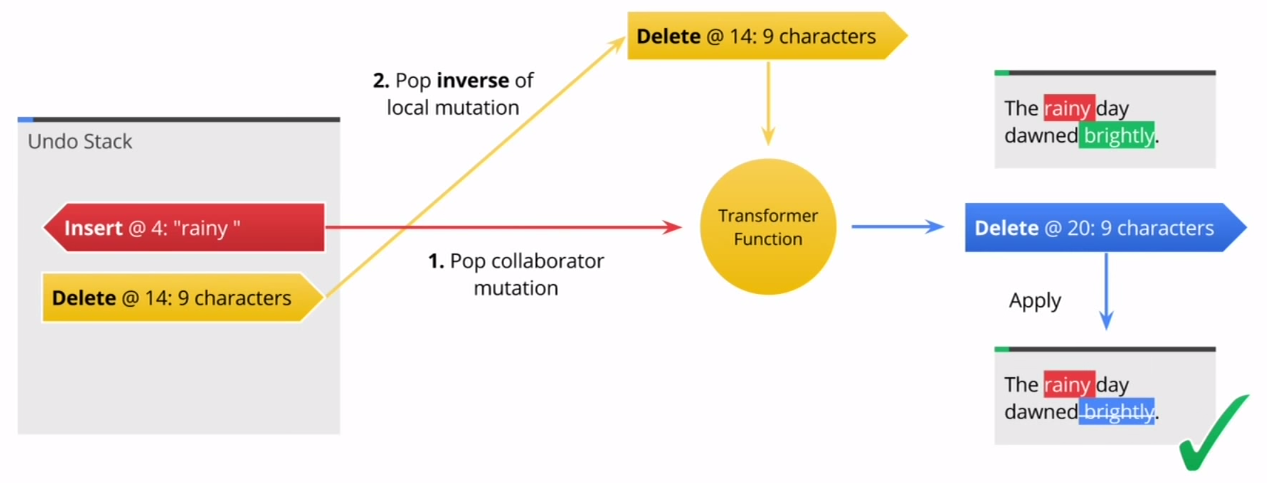
\includegraphics[width=\textwidth]{images/ot_transform_redo.png}
	\caption{For the undo, local changes need to be transformed against remote changes by the transformer \cite{website:io2013-drive-api-video}}
\end{figure} 

\section{\TeX and \LaTeX}
\label{sec:tex}

\TeX is a typesetting system that was invented by Donald E. Knuth in the late 1970s \cite{website:knuth}. It is specifically used for math, technical and other scientific publications, as it contains innumerable amounts of symbols and formulas used in this area, and allows to set the type in outstanding accuracy and quality. It was ultimately developed for Knuth's book series \name{The Art of Computer Programming} and consists of an independent computer programming language and a macro compiler whose source codes were published by Knuth in a computer and operating system independent form \cite{website:tug}.

The output format of a typeset document is \name{DeVice Independent} (\abk{DVI}{DeVice Independent}) and contains positioning directives, references to fonts, type and lines. It is stored, as already stated by the file name, in an device independent form. Before viewing or printing, this format must then be converted into the format of the respective output device, which is nowadays typically a \name{Portable Document File} (\abk{PDF}{Portable Document File}).

As \LaTeX itself is only a macro compiler with relatively few directives that are not sufficiend for most use cases, a set of other macros is needed. Among the most popular set of such macros is \LaTeX which was originally created by Leslie E. Lamport and can be extended by myriads of additional packages \cite{website:dante}.

\pagebreak

The basic macros provide some pre-defined document classes such as article, book, report and slides. There are then possiblibities to structure them further in chapters or sections, with hyperreferences, bibliography, citations, abbreviations and more.

For the conversion to the format of the respective output device, there are so-called engines executing the \TeX format. For example, \LaTeX can be used under \name{PDFTex} as well as under the engines \name{LuaTex} and \name{XeTex}. Although the former is probably the most used, these two are its successors and while \name{XeTex} is considered to be slightly more stable than \name{LuaTex} at the moment, its extensibility might be surpassed by it in the near future.
